\documentclass[../../main.tex]{subfiles}
\begin{document}

\noindent
{\bf [解1]} 以下 $t = \cos\theta, s = \sin\theta$ とする. $P$ の座標は $P(at, bs, c+1)$ とおける. この $P$ からの光が与える影は, 四角形であり, $A(a,b), B(a,-b), C(-a,b), D(-a,-b)$ とおき, $PA, PB, \dots, PD$ と $xy$ 平面の交点を $A', B', C', D'$ とおく. 四角形 $A'B'C'D'$ になる. 相似から $K = A, B, C, D$ に対して
\[
  \vec{PK'} = (c+1)\vec{PK}
\]
となり,
\[
  \vec{PA'} = (c+1)
  \begin{pmatrix} a - at \\ b - bs \\ c - (c+1)
  \end{pmatrix} = (c+1)
  \begin{pmatrix} a(1-t) \\ b(1-s) \\ -1
  \end{pmatrix}
\]
\[
  \vec{PB'} = (c+1)
  \begin{pmatrix} a(1-t) \\ -b(1+s) \\ -1
  \end{pmatrix}, \quad \vec{PC'} = (c+1)
  \begin{pmatrix} -a(1+t) \\ b(1-s) \\ -1
  \end{pmatrix}, \quad \vec{PD'} = (c+1)
  \begin{pmatrix} -a(1+t) \\ -b(1+s) \\ -1
  \end{pmatrix}
\]
となり
\[
  A'\big( a(c+1) - act, b(c+1) - bcs, 0 \big), \quad C'\big( -a(c+1) - act, b(c+1) - bcs, 0 \big)
\]
\[
  B'\big( a(c+1) - act, -b(c+1) - bcs, 0 \big), \quad D'\big( -a(c+1) - act, -b(c+1) - bcs, 0 \big)
\]
だから, $\theta$ を固定した時の影は右図斜線部. ただし $E(-act, -bcs, 0)$ とした. $\theta$ をうごかすと, $E$ は, 楕円
\[
  \dfrac{x^2}{a^2} + \dfrac{y^2}{b^2} = c^2, \quad z=0
\]
の上をきれ目なく動くから, 影の通過領域は右下図斜線部. この面積 $T$ は，楕円，中央の長方形，周囲の長方形に分けて，
\begin{align}
  T & = abc^2 \pi + 4ab(c+1)^2 + 2 \cdot ac \cdot 2b(c+1) + 2 \cdot bc \cdot 2a(c+1) \\
  & = \big( \pi c^2 + 4(c+1)(3c+1) \big) ab
\end{align}

\begin{figure}[H]
  \centering
  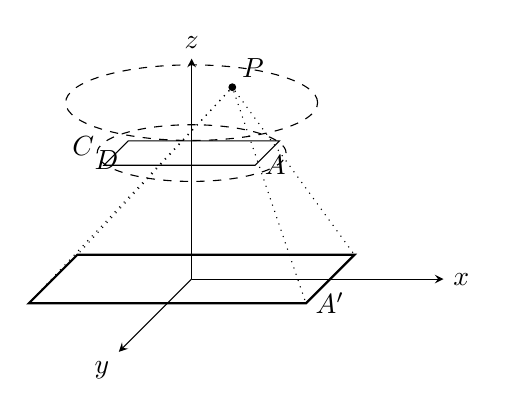
\begin{tikzpicture}[scale=0.8, >=stealth]
    % 3D perspective projection diagram
    \draw[->] (0,0,0) -- (4,0,0) node[right] {$x$};
    \draw[->] (0,0,0) -- (0,3.5,0) node[above] {$z$};
    \draw[->] (0,0,0) -- (0,0,3) node[below left] {$y$};

    \draw[dashed] (0,2.8,0) ellipse (2cm and 0.6cm);
    \node[circle, fill, inner sep=1pt] (P) at (0.8, 3.2, 0.4) {};
    \node[above right] at (P) {$P$};

    \draw[dashed] (0,2.0,0) ellipse (1.5cm and 0.45cm);
    \coordinate (A) at (1.2, 2.0, 0.5);
    \coordinate (B) at (1.2, 2.0, -0.5);
    \coordinate (C) at (-1.2, 2.0, 0.5);
    \coordinate (D) at (-1.2, 2.0, -0.5);
    \draw (A) -- (B) -- (D) -- (C) -- cycle;
    \node[right] at (A) {$A$};
    \node[above left] at (C) {$C$};
    \node[below left] at (D) {$D$};

    \coordinate (A') at (2.2, 0, 1.0);
    \coordinate (B') at (2.2, 0, -1.0);
    \coordinate (C') at (-2.2, 0, 1.0);
    \coordinate (D') at (-2.2, 0, -1.0);
    \draw[thick] (A') -- (B') -- (D') -- (C') -- cycle;
    \node[right] at (A') {$A'$};

    \draw[dotted] (P) -- (A');
    \draw[dotted] (P) -- (B');
    \draw[dotted] (P) -- (C');
    \draw[dotted] (P) -- (D');
  \end{tikzpicture}
  \qquad
  \begin{tikzpicture}[scale=0.7, >=stealth]
    % Fixed theta shadow box
    \draw[->] (-2.5, 0) -- (2.5, 0) node[right] {$x$};
    \draw[->] (0, -2.5) -- (0, 2.5) node[above] {$y$};

    \fill[pattern=north east lines, pattern color=gray!60] (-1.5, -1.5) rectangle (1.5, 1.5);
    \draw[thick] (-1.5, -1.5) rectangle (1.5, 1.5);

    \node[above right] at (1.5, 1.5) {$A'$};
    \node[below right] at (1.5, -1.5) {$B'$};
    \node[above left] at (-1.5, 1.5) {$C'$};
    \node[below left] at (-1.5, -1.5) {$D'$};

    \fill (0.2, 0.3) circle (1.5pt) node[below left] {$E$};
    \node[above right] at (1.5, 1.5) {\footnotesize $a(c+1)$};
    \node[right] at (1.5, 0.8) {\footnotesize $b(c+1)$};
  \end{tikzpicture}
  \caption{点光源による射影と，角度を固定したときの影}
  \label{fig:1}
\end{figure}

\begin{figure}[H]
  \centering
  \begin{tikzpicture}[scale=0.75, >=stealth]
    % Envelope region T
    \draw[->] (-3.5, 0) -- (3.5, 0) node[right] {$x$};
    \draw[->] (0, -3.5) -- (0, 3.5) node[above] {$y$};

    \fill[pattern=north east lines, pattern color=gray!60]
    (1.5, 2.5) -- (-1.5, 2.5)
    arc (90:180:1.0cm and 1.0cm) -- (-2.5, -1.5)
    arc (180:270:1.0cm and 1.0cm) -- (1.5, -2.5)
    arc (270:360:1.0cm and 1.0cm) -- (2.5, 1.5)
    arc (0:90:1.0cm and 1.0cm) -- cycle;

    \draw[thick] (1.5, 2.5) -- (-1.5, 2.5);
    \draw[thick] (-2.5, 1.5) -- (-2.5, -1.5);
    \draw[thick] (-1.5, -2.5) -- (1.5, -2.5);
    \draw[thick] (2.5, -1.5) -- (2.5, 1.5);

    \draw[thick] (1.5, 1.5) ++(1.0,0) arc (0:90:1.0cm and 1.0cm);
    \draw[thick] (-1.5, 1.5) ++(0,1.0) arc (90:180:1.0cm and 1.0cm);
    \draw[thick] (-1.5, -1.5) ++(-1.0,0) arc (180:270:1.0cm and 1.0cm);
    \draw[thick] (1.5, -1.5) ++(0,-1.0) arc (270:360:1.0cm and 1.0cm);

    \draw[dashed] (-1.5, -1.5) rectangle (1.5, 1.5);
    \draw[dashed] (0,0) ellipse (1.0cm and 1.0cm);

    \node[below right] at (0,0) {$0$};
    \node[right] at (2.5, 0.5) {\footnotesize $a(2c+1)$};
    \node[below] at (1.5, 0) {\footnotesize $a(c+1)$};
    \node[above right] at (1.0, 0) {\footnotesize $ac$};
    \node[left] at (-1.0, 0) {\footnotesize $-ac$};

    \node[above] at (0, 2.5) {\footnotesize $b(2c+1)$};
    \node[right] at (0, 1.5) {\footnotesize $b(c+1)$};
    \node[above right] at (0, 1.0) {\footnotesize $bc$};
    \node[below] at (0, -1.0) {\footnotesize $-bc$};
    \node[below] at (0, -2.5) {\footnotesize $-b(2c+1)$};
  \end{tikzpicture}
  \caption{影が通過する領域}
  \label{fig:2}
\end{figure}

\bigskip

\noindent
{\bf [解2]} ($\theta$ において $P$ の座標を仮定した後)

\noindent
点 $Q(X, Y, 0)$ が領域内の点だとすると, 直線 $PQ$ と長方形の板が共有点を持つ.
\[
  \vec{PQ} =
  \begin{pmatrix} X \\ Y \\ 0
  \end{pmatrix} -
  \begin{pmatrix} at \\ bs \\ c+1
  \end{pmatrix}
\]
だから, $PQ$ 上の点 $R$ は,
\[
  \vec{OR} =
  \begin{pmatrix} X \\ Y \\ 0
  \end{pmatrix} + d
  \begin{pmatrix} -X + at \\ -Y + bs \\ c+1
  \end{pmatrix}
\]
で表されるから, $z=c$ の時, $d = \dfrac{c}{c+1}$ ($\equiv d_0$) として,
\[
  R\Big( (1-d_0)X + a d_0 t, (1-d_0)Y + b d_0 s, c \Big)
\]
である. これが長方形内部なら良いので, $1-d_0 = \dfrac{1}{c+1}$, $a, b > 0$ に注意して,
\[
  \begin{cases}
    \left| \dfrac{1}{c+1} X + a d_0 t \right| \le a \\[10pt]
    \left| \dfrac{1}{c+1} Y + b d_0 s \right| \le b
  \end{cases}
  \iff
  \begin{cases}
    -a d_0 t - a \le \dfrac{1}{c+1} X \le -a d_0 t + a \\[10pt]
    -b d_0 s - b \le \dfrac{1}{c+1} Y \le -b d_0 s + b
  \end{cases}
  \quad \dots \phi
\]
$\phi$ を図示すると, 右図斜線部である. ただし, $x = \dfrac{X}{c+1}, y = \dfrac{Y}{c+1}$ とした. したがって $\phi$ を動かせば [解1] と同様の領域をえがくことが出来る.

\begin{figure}[H]
  \centering
  \begin{tikzpicture}[scale=0.7, >=stealth]
    \draw[->] (-3, 0) -- (3, 0) node[right] {$x$};
    \draw[->] (0, -2.5) -- (0, 2.5) node[above] {$y$};

    \draw[dashed] (0,0) ellipse (1.8cm and 1.2cm);
    \fill (1.4, 0.7) circle (1.5pt) node[above right] {\footnotesize $b d_0$};
    \node[above right] at (1.8, 0) {\footnotesize $a d_0$};

    \fill[pattern=north east lines, pattern color=gray!60] (-1.2, -0.8) rectangle (1.2, 0.8);
    \draw[thick] (-1.2, -0.8) rectangle (1.2, 0.8);

    \node[below left] at (-1.2, 0) {\footnotesize $-a$};
    \node[below right] at (1.2, 0) {\footnotesize $a$};
    \node[above left] at (0, 0.8) {\footnotesize $b$};
    \node[below left] at (0, -0.8) {\footnotesize $-b$};
    \node[below left] at (0,0) {\footnotesize $0$};
  \end{tikzpicture}
  \caption{解2で得られる不等式の領域}
  \label{fig:3}
\end{figure}

\end{document}
